In this section we provide an implementation of a patrol script for an entity in a game. The sample is made up of an entity, representing a guard, and a couple of checkpoints. The guard continuously moves between the two checkpoints. We choose this sample because this is a typical behaviour implemented in several games, where the user is able to set up a patrol route for a unit.
Below we provide the code for the patrol logic in a ``prettified'' version of Casanova 2.5, that is, using a syntax to get rid of all the additional structures used by the metacompiler for the rule evaluation. This syntax can be made available by using a parser which then produces either the corresponding syntax in the metacompiler or directly the metacompiler AST. We choose to ignore this step because its solution is known in literature and trivial.

\begin{lstlisting}
rule Position = Position + Velocity * dt

rule Velocity =
  wait Position.X >= 300f || Position.X <= 0f
  yield new Vector2(-Velocity.X, 0f)
\end{lstlisting}

In the following section we show the comparison between the sample implemented in Casanova 2.5 and an equivalent implementation in Python with respect to the running time. We then show a comparison between the hard-coded compiler of Casanova 2.0 and the implementation of Casanova 2.5 in Metacasanova with respect to the code length. We want to underline that the main goal of this work is \textbf{to ease the process of building a compiler for a DSL for games, thus our main objective is decreasing the code length and complexity necessary to implement a hard-coded compiler for the language}. At the same time we show that the compiled program in Casanova 2.5 \textbf{has performance similar to that of a language used in game development, and thus Casanova 2.5 is usable in a real scenario}.

\subsection{Chosen languages}
We compared the running time of the sample in metacompiled Casanova with an equivalent implementation in Python. This language was chosen based on its use in game development: Python has been used extensively in several games such as Civlization IV \cite{CIV4} or World in Conflict \cite{WIC} because of the native support for coroutines. Furthermore we decided on purpose not to compare the performance of the same game in C++ and C\#, although they are widely used in the industry, because we knew in advance \cite{CASANOVA2_PAPER} that the current version of the code generated by the meta-compiler would not match the high performance of these languages. The sample has been run with a number of entities ranging from 100 to 1000 for 100 game state updates. An average update time was determined afterwards based on the total running time of the game logic update.


\subsection{Performance}
The performance results are shown in Table \ref{tab:evaluation} and Figure \ref{fig:evaluation}. We see that the generated code has performance on the same order as Python. This is mainly due to the fact that the memory, in the metacompiled implementation of Casanova, is managed through a map, and because of the virtuality of the implemented operators. Each time Casanova accesses a field in an entity this must be looked up into the map. To this we add the complexity of dynamic lookups when we must deal with polymorphic results into the rules. 

From Table \ref{tab:compiler_comparison} we see that the implementation of Casanova 2.0 language in Metacasanova is almost 5 times shorter in terms of lines of code than the previous Casanova implementation in F\#. We believe it is worthy of notice that structures with complex behaviours, such as \textit{wait} or \textit{when}, require hundreds of lines of codes with a standard approach (the code lines to define the behaviour of the structure plus the support code to correctly generate the state machine), while in the meta-compiler we just need tens of lines of codes to implement the same behaviour. Moreover we want to point out that the previous Casanova compiler was written in a functional programming language: this languages tend to be more synthetic than imperative languages, so the difference with the same compiler implemented in languages such as C/C++ might be even greater.

The readability with respect to the hard-coded compiler code is also improved: we managed to implement the behaviour of synchronization and timing primitives almost imitating one to one the formal semantics of the language definition. In the hard-coded compiler implementation for Casanova 2.0 the semantics is lost in the code for generating finite state machines.

\begin{figure}
	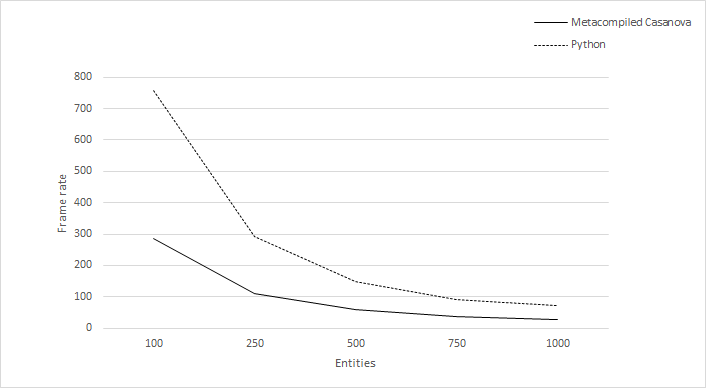
\includegraphics[scale = 0.4]{Charts/evaluation}
	\caption{Performance comparison}
	\label{fig:evaluation}
\end{figure}

\begin{table}
	\begin{tabular}{|c|c|c|}
		\hline
		\multicolumn{3}{|c|}{\textbf{Casanova 2.5}} \\
		\hline
		Entity \# & Average update time (ms) & Frame rate \\
		\hline
		100 & 0.00349 & 286.53 \\
		\hline
		250 & 0.00911 & 109.77 \\
		\hline
		500 & 0.01716 & 58.275 \\
		\hline
		750 & 0.02597 & 38.506 \\
		\hline
		1000 & 0.03527 & 28.353 \\
		\hline
		\multicolumn{3}{|c|}{\textbf{Python}} \\
		\hline
		Entity \# & Average update time (ms) & Frame rate \\
		\hline
		100 & 0.00132 & 756.37 \\
		\hline
		250 & 0.00342 & 292.05 \\
		\hline
		500 & 0.00678 & 147.54 \\
		\hline
		750 & 0.01087 & 91.988 \\
		\hline
		1000 & 0.01408 & 71.002 \\
		\hline
	\end{tabular}
	\caption{Patrol sample evaluation}
	\label{tab:evaluation}
\end{table}

\begin{table}
	\begin{tabular}{|c|c|}
		\hline
		\multicolumn{2}{|c|}{\textbf{Casanova 2.5 with Metacasanova}} \\
		\hline
		Module & Code lines \\
		\hline
		Data structures and function definitions & 40 \\
		\hline
		Query Evaluation & 16 \\
		\hline
		While loop & 4 \\
		\hline
		For loop & 5 \\
		\hline
		If-then-else & 4 \\
		\hline
		When & 4 \\
		\hline
		Wait & 6 \\
		\hline
		Yield & 10 \\
		\hline
		Additional rules for Casanova program evaluation & 40 \\
		\hline
		Additional rules for basic expression evaluation & 201 \\
		\hline
		\multicolumn{2}{|l|}{\textbf{Total: } 300} \\
		\hline
		\multicolumn{2}{|c|}{\textbf{Casanova 2.0 compiler}} \\
		\hline
		Module & Code lines \\
		\hline
		While loop & 10 \\
		\hline
		For-loop and query evaluation & 44 \\
		\hline
		If-Then-Else & 15 \\
		\hline
		When & 11 \\
		\hline
		Wait & 24 \\
		\hline
		Yield & 29 \\
		\hline
		Additional structures for rule evaluation & 63 \\
		\hline
		Structures for state machine generations & 754 \\
		\hline
		Code generation & 530 \\
		\hline
		\multicolumn{2}{|l|}{\textbf{Total: } 1480} \\
		\hline			
	\end{tabular}	
	\caption{meta-compiler vs standard compiler}
	\label{tab:compiler_comparison}
\end{table}